
\chapter{Fundamental equations of turbomachinery}

\section{Basics and principles}
\subsection{Introduction}
	About the exam, he likes the drawings and likes to give a sentence and asks if it is the reality or not. The questions are about the \textbf{lectures} and not the notes. This summary is thus mainly based on the lectures. \\

The course is organized as: 

\begin{enumerate}
\item \textbf{Turbopumps} and the system involved: a pump is something  applying pressure to a fluid $\Delta p > 0$, which will first be a liquid $\rho = cst$.

\item \textbf{Turbines:} in this case the fluid involves a pressure loss $\Delta p < 0$, so expansion (a valve, simple releaser). We will see the gas turbines and the hydraulic turbines. Some machines can be used in the two ways, both roles, same mechanical component is acting as a pump and as a turbine in the other direction (reversible). 

\item \textbf{Volumetric compressors:} as in other courses we have polytropic or isentropic efficiency, we can define volumetric compressors. 

\item \textbf{Compressors} $\bm{\rho \neq cst}$: we need to consider the axial and centrifugal systems separately because they are very different and complicated.   
\end{enumerate}


\subsection{Classification of turbomachines}
If the role of the machine is to extract energy from the fluid to the shaft we speak about \textbf{turboproducers} or \textbf{turbomotors} (ex: hydraulic turbines), and in the other case \textbf{turboabsorbers} or \textbf{turbogenerators}. 

\subsection{General organization of turbomachines}
\wrapfig{6}{l}{4}{0.22}{ch1/1} 
We always have a \textbf{shaft}, and on the shaft we have a \textbf{disk} or a \textbf{rotor} where the energy transformation takes place, and on this we put a \textbf{blade} (white rectangle on \autoref{ch1/1}), an element with a given geometry. The blade is situated at a distance $r_H$ from the shaft and implies high tangential velocities. The device is closed by a \textbf{carter} and we have to be careful at the top of the blade since there can be leakage, this is why the clearance is very small ($\mu m$). We can also have active clearance control by blowing fluid on the carter. Remark that there is an \textbf{external carter} (blue 1) and an \textbf{internal carter} (blue 2) that can constitute a convergent distributor and a divergent diffuser. These can contain non rotating parts called \textbf{vane}, we speak of \textbf{vaned convergent}, \textbf{vaned divergent} or \textbf{vaneless} nozzles. The internal carter plays the role of support and is connected to the shaft via \textbf{bearings} and \textbf{seals} (to avoid air preferring this way to reach atmospheric pressure). 

\ \\
\begin{wrapfigure}[7]{l}{4.5cm}
\vspace{-10mm}
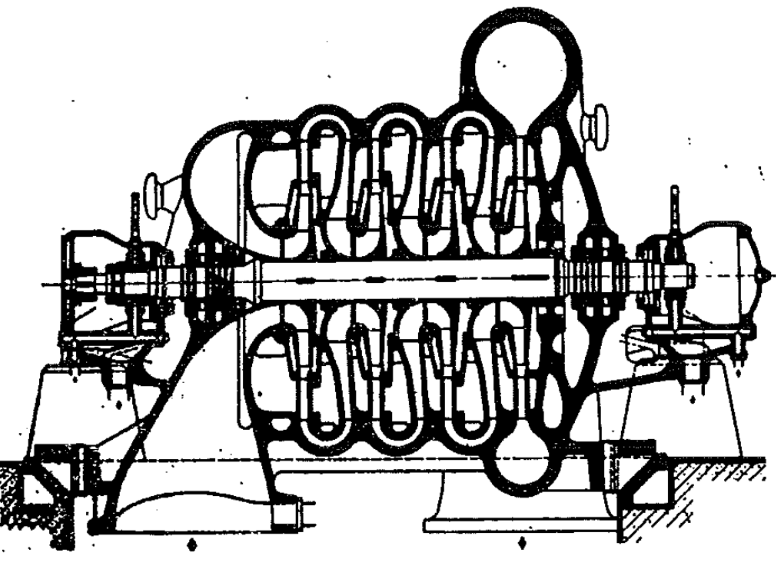
\includegraphics[scale=0.3]{ch1/2}
\captionof{figure}{}
\label{ch1/2}
\end{wrapfigure}
The major types of machine have an axial configuration so that the particles flows parallel to the shaft, radial configuration where flows enters horizontal and leaves vertical also exists. Most turbines or compressors are axial turbines. Turbopumps are most of the time radial, centrifugal. Several disks can be mounted on a same shaft (or several shafts), with fixed components changing the direction of the flow (multistage pump on \autoref{ch1/2}).

\subsection{Notations}
On \autoref{ch1/1}, 0 is the inlet of the distributor, 1 the inlet of the rotor, 2 outlet of the rotor, 3 outlet of the diffuser and i (or e)/o (or s) the upstream/downstream plenum. There are 3 velocity components: the absolute velocity $\bar{v}$, the frame tangential velocity $\bar{u}$ and the relative velocity $\bar{w}$ due to the rotation of fluid particles. 

\subsection{Velocity triangle}
\wrapfig{8}{r}{3.5}{0.3}{ch1/3}
The absolute velocity respects: 

\begin{equation}
\bar{v} = \bar{u} + \bar{w}.
\end{equation}

By defining $\alpha$ and $\beta$ the angle between $\bar{u}$ and respectively $\bar{v}$ and $\bar{w}$, we can write: 

\begin{equation}
v \cos \alpha = u + w\cos \beta \qquad w^2 = u^2 + v^2 - 2uv\cos \alpha
\end{equation}

The velocity triangle is the keypoint of a turbomachine, we have to play with the velocities by means of the mass flow rate $\dot{m}$ and the machine rpm $N$. It is important to see that these parameters are linked to the velocity triangle, for the mass flow for example $\dot{m} = \rho u A$. 


\section{Fundamental equations of the flow}
\subsection{Equations of the flow in a fixed frame}
For all developments, only \textbf{steady state} regime is considered, so that $\omega = cst$ and the flow properties are not time dependent. Moreover, boundary layers are neglected and the flow propagates in parallel slices. 

\subsubsection{Energy equation}
Let's consider sections $A_0$ and $A_1$ denoting the input and output of a non interrupted flow section, for instance 0 to 1 in previous figure. The total energy equation is: 

\begin{equation}
q = h_1 - h_0 + \frac{v_1^2 - v_0^2}{2} + g(z_1-z_0)
\label{2.1}
\end{equation}

where $q$ is the heat exchanged with the outside [J/kg], $v$ is the absolute velocity [m/s] and $h$ is the enthalpy [J/kg]. In adiabatic systems $q=0$. We see that if there is thermal, kinetic or potential energy loss, it will produce heat. Be careful that this equation is not applicable around the blade. 

\subsubsection{Equation of kinetic energy}
We know that kinetic and potential energy can be transformed into work in a machine. We have:

\begin{equation}
 \frac{v_1^2 - v_0^2}{2} + g(z_1-z_0) = - \int _{p_0}^{p_1} \nu dp - w'_f
 \label{2.2}
\end{equation}

where $\nu = 1/\rho$ is the specific volume [$m^3$/kg] and $w'_f$ the work resulting from all friction effects [J/kg]. We see that if velocity increases/decreases, pressure decreases/increases and the friction is a loss, so "-" signs. 

\subsubsection{Global thermodynamic equation}
By considering \eqref{2.2} in \eqref{2.1}: 

\begin{equation}
q + w'_f = h_1 - h_0  - \int _{p_0}^{p_1} \nu dp
\end{equation}

The physical content is different, we see that in fact the losses corresponds to pressure and temperature losses. 

\subsubsection{Mass flow rate equation}
The mass flow is constant over a tube: 

\begin{equation}
\dot{m} = \rho v A = \rho_0 v_0 A_0 = \rho_1 v_1 A_1 = \frac{v_1 A_1}{\nu _1}  
\end{equation}

where $\dot{m}$ [kg/s].

\subsection{Equations of the flow in a moving frame}
Now we can consider the indices 1 and 2 referring to the blade space. 

\subsubsection{Equation of kinetic energy in a relative space}
He skipped the long demo page 8. The equations are the same as before, the only difference is that we replace the absolute velocity by the relative one and an additional kinetic energy term due to the rotation of the frame: 

\begin{equation}
 \frac{w_2^2 - w_1^2}{2} + g(z_2-z_1) = - \int _{p_1}^{p_2} \nu dp - w^"_f + \frac{u_2^2-u_1^2}{2}
 \label{2.5}
\end{equation}

Remark that this term can play a huge role because in a centrifugal system the term is non zero while it is zero in an axial system. 

\subsubsection{Global thermodynamic equation}
The equation is exactly the same as before, except $w'_f$ that becomes $w^"_f$. 
\begin{equation}
q + w^"_f = h_2 - h_1 - \int _{p_1}^{p_2} \nu dp
\end{equation}

\subsubsection{Energy equation}
If we combine the two previous equation we get: 

\begin{equation}
q + \frac{u_2^2-u_1^2}{2} = h_2 - h_1 + \frac{w_2^2 - w_1^2}{2} + g(z_2-z_1)
\end{equation}

\subsubsection{Mass flow equation rate equation}
For a section normal to the relative velocity:

\begin{equation}
\dot{m} = \rho w A = \rho _1 w_1 A_1 = \rho _2 w_2 A_2
\end{equation}


\section{Fundamental equations of turbomachinery}
\subsection{Compressors}
\subsubsection{Internal losses}
\wrapfig{8}{l}{5}{0.3}{ch1/4}
Several kind of losses are present in a compressor. First of all, friction in the distributor gives birth to losses noted $w'_f$. Then, the fluid goes through the interblade channel where its energy increases, but a loss due to friction is present $w^"_f$. In addition, the clearance between the blade tip and the carter is non zero and leads to back-flow leakage $\dot{m}_i$ as the pressure upstream is lower. If we denote the mass flow rate through the blades $\dot{m}_R$, we have: 

\begin{equation}
\dot{m}_R = \dot{m} + \dot{m}_i
\end{equation}

A big part of the flow goes then through the diffuser, but a small part escapes from the seal to the outside $\dot{m}_e$. The small gap between the rotor and the internal carter is filled with part of the fluid. Even if this fluid does not contribute to the energy exchanges (stagnation), part of the power supplied to the shaft will dissipate due to fluid friction $P_{fr}$. 

\subsubsection{External losses}
As discussed, part of the flow escapes through the seals. The upstream one is not a problem since the pressure is close to the atmospheric pressure, but for the downstream seal $\dot{m}_e \neq 0$ since the pressure is higher. This will be neglected in the study. The last losses are due to bearings and other mechanical components such as the fuel pump that we all denote in a single absorbed power $P_{fa}$. 

\subsubsection{Energy equation}
\wrapfig{10}{l}{6.5}{0.3}{ch1/7}
Before going through all the losses appearing in the engine, let's have a global view limiting the study region as on the figure. The total energy equation between input and output is: 

\begin{equation}
q + W_{e\rightarrow s} = u_o - u_i + \frac{v_o ^2 - v_i^2}{2} + g(z_o - z_i)
\end{equation}

where we have the heat exchanged with the outside, the work from external forces to the system due to fluid pressure $p_i \nu _i - p_o\nu_o$ and work applied on the shaft $\frac{P - P_{fa}}{\dot{m}} =  \frac{P_i}{\dot{m}}$ equal to the variation of internal energy, kinetic energy and potential energy. Heat exchanges and the height difference in such engine are negligible, by introducing the enthalpy instead of internal energy and fluid pressure, we have: 

\begin{equation}
P_i = P - P_{fa} = \dot{m}\left( h_o - h_i + \frac{v_o^2 - v_i^2}{2} \right) = \dot{m} (h_{t_o} - h_{t_i}) = \dot{m} c_p (T_{t_o} - T_{t_i})
\end{equation}

where the index $t$ denotes the total or stagnation quantities. We conclude that the work transferred through the shaft increases the total energy of the fluid. 

\subsubsection{Equation of kinetic energy}
This adapted to the work $\frac{P_i}{\dot{m}}$ gives: 

\begin{equation}
P_i = \dot{m} \underbrace{\left( \frac{v_o^2-v_i^2}{2} + \int _{i}^{o} \nu dp + g(z_o - z_i)\right)}_{e} + P_f = \dot{m} e + P_f
\end{equation}

$P_f$ is the internal friction loss with the active as well as the non-active fluid and $e$ is the energy transferred to the fluid. 

\subsubsection{A first distribution of the power - efficiencies}
\wrapfig{7}{r}{3.2}{0.3}{ch1/8}
The figure summarizes all the above equations, for the efficiency we have $\dot{m}e$ at the end and we inject $P$ so: 

\begin{equation}
\eta _{g} = \frac{\dot{m}e}{P} = \frac{\dot{m}e}{P_i} \frac{P_i}{P} = \eta _i \eta _m
\end{equation}

that we rewrite as internal efficiency and external mechanical efficiency. 

\subsubsection{Energy transfer to the rotor}
The only new equation we have is the \textbf{Euler-Rateau equation}. The energy given to the flow in a pump is linked to the energy provided to the shaft. We have to consider the kinetic moment (moment of the quantity of movement) related to the shaft:

\begin{equation}
\frac{d}{dt}\sum M_{axe} (m\bar{v}) = \sum M_{axe}\bar{F}_e
\label{3.2}
\end{equation}

\wrapfig{11}{l}{3}{0.3}{ch1/5}
The variation of the kinetic moment of the rotor is zero since the rotation speed is constant. For a fluid element with mass $m$ and at a distance $r$ of the shaft, the velocity $\bar{v}$ is composed of a component // to the shaft, radial component and tangential component on the rotor. Only the tangential component delivers a moment: 

\begin{equation}
M_{axe}(m\bar{v}) = m r v \cos \alpha 
\end{equation}

and since the flow is permanent, after a time $dt$ very small, if the mass flow is constant: 

\begin{equation}
\sum _{b'b^"} mr v \cos \alpha - \sum _{a'a^"} mr v \cos \alpha = m' (r_2v_2\cos \alpha _2-r_1v_1\cos \alpha _1) = m' (r_2 v_{2u} - r_1 v_{1u})
\end{equation}

Accepting $r_2 v_{2u} - r_1 v_{1u} = cst$ for all channels we get: 

\begin{equation}
\frac{d}{dt}\sum M_{axe}(m\bar{v}) = \frac{d}{dt}\left[(r_2 v_{2u} - r_1 v_{1u}) \sum m'\right] = \dot{m}_R (r_2 v_{2u} - r_1 v_{1u})
\end{equation}

For the right hand side of \eqref{3.2}, the weight of the wheel, the weight of the fluid, the pressures at inlet, at outlet and at side walls are null due to symmetry. Only the \textbf{driving torque} applied on the shaft $\bf{M_i}$ and the \textbf{resistive torque} $-\bf{M_{fr}}$ due to friction between the wheel and the non-active fluid are present, so that we finally get: 

\begin{equation}
\dot{m}_R (r_2 v_{2u} - r_1 v_{1u}) = M_i - M_{fr}
\end{equation}

And if we multiply by $\omega$: 

\begin{center}
\theor{
\textbf{Equation of Euler-Rateau}
\begin{equation}
P_i - P_{fr} = P - P_{fa} - P_{fr} = P_R = \dot{m}_R (u_2 v_{2u} - u_1 v_{1u}) = \dot{m}_R \Delta (uv_u)
\end{equation}
This equation tells that in order to be transferred to the mass flow rate $\dot{m}_R$, the power at the rotor shaft $P_R$ must show an increase of the quantity $uv_u$ which is directly related to the velocity triangle. 
}
\end{center}

As $w^2 = v^2 + u^2 - 2 u v_u$, one can also write: 

\begin{equation}
P_R = \dot{m}_R \left( \frac{v_2 ^2 - v_1^2}{2} + \frac{u_2 ^2 - u_1^2}{2} - \frac{w_2 ^2 - w_1^2}{2} \right)
\label{3.8}
\end{equation}

\subsubsection{Energy generated by the rotor}
Remember \eqref{2.5} and replace this in \eqref{3.8}, we get: 

\begin{equation}
P_R = \dot{m}_R \underbrace{\left( \frac{v_2 ^2 - v_1^2}{2}  + \int _{p_1}^{p_2} \nu dp + g(z_2 - z_1) \right)}_{e_R} + \dot{m} _R w^"_f
\end{equation}

where $e_R$ is the energy transferred to the fluid through the channels on the rotor between section 1 and 2 on the common figure. $\dot{m}_R w^"_f = P^"_f$ being the power absorbed by friction effects, we get: 

\begin{center}
\theor{
\begin{equation}
P_R = \dot{m}_Re_R + P^"_f \qquad \left(\mbox{and } P_R = \dot{m} (h_{t_2} - h_{t_1}) \right)
\end{equation}
}
\end{center}

And we get thus 4 different expression for $P_R$, where the last expression was given in lecture. 

\subsection{Detailed power distribution}
The different losses can be depicted thanks to the previous equation:

\begin{equation}
P_i = P-P_{fa} \qquad P_R = P_i - P_{fr} \qquad \dot{m}_Re_R = P_R - P^"_{f} \qquad \dot{m}_R = \dot{m} + \dot{m}_i
\end{equation}

\wrapfig{12}{l}{5}{0.3}{ch1/6}
where we clearly see the mechanical losses, the loss due to stationary fluid, the loss at the rotor and the back flow. To this we have to add the loss at the diffuser and distributor which we wrote as:

\begin{equation}
P'_f = \dot{m}w'_f
\end{equation}

On the figure, we first see the loss due to mechanical components giving $P_i$, then the fluid losses composed of stationary fluid losses giving $P_R$, then rotor channels loss giving $\dot{m}_Re_R$, but we have the back flow loss $\dot{m}_i e_R$ giving $\dot{m}e_R$ and the last venturi losses that gives the output power $\dot{m}e$ plus all the losses. 

\section{Turbines}
\subsubsection{Description}
\wrapfig{11}{r}{4.5}{0.3}{ch1/9}
The equations are in fact the same except that we have to adapt the signs and indexes to the working principle since the energy is flowing from the fluid to the shaft. As before, there is a clearance flow $\dot{m}_i$ such that: 

\begin{equation}
\dot{m} = \dot{m}_R + \dot{m}_i
\end{equation}

The losses due to mechanical components $P_{fa}$ and the leakage flows $\dot{m}_e$ (negligible), the energy losses in non rotating ($w'_f$) and rotating ($w^"_f$) frame and the loss due to non-active fluid $P_{fr}$ are present. The useful power $P_u$ replaces the $P$ we had before. 

\subsubsection{Energy equation}
It is the same as before except that the indexes are inverted and the useful power is $P_u = P_i - P_{fa}$:

\begin{equation}
P_i = P_u + P_{fa} = \dot{m} (h_{t_i} - h_{t_o})
\end{equation} 

\subsubsection{Equation of kinetic energy}
\begin{equation}
P_i = \dot{m} \underbrace{\left( \frac{v_i^2-v_o^2}{2} + \int _{p_o}^{p_i} \nu dp + g(z_i - z_o)\right)}_{e} - P_f = \dot{m} e - P_f
\end{equation}

\subsubsection{First distribution of the power}
The efficiencies are inverted: 

\begin{equation}
\eta _g = \frac{P_u}{\dot{m}e} = \frac{P_u}{P_i}\frac{P_i}{\dot{m}e} = \eta _m \eta _i
\end{equation}

On \autoref{ch1/10} is represented a first plot of the different powers, remark that it is similar to what we had, only the fluid losses comes before the mechanical losses. The fluid losses are the same as before. 

\minifig{ch1/10}{ch1/11}{0.4}{0.27}{0.35}{0.35}

\subsubsection{Equation of Euler-Rateau}
We can rewrite $P_R$ as the power transfered to the rotor from the fluid $\dot{m}_R$: 

\begin{equation}
P_R = P_i + P_{fr} = \dot{m} _R (u_1v_1\cos \alpha _1 - u_2v_2\cos \alpha _2) 
\end{equation}

\subsubsection{Energy absorbed by the rotor}
As before, combing the above equation and the equation for rotating frame we get: 

\begin{equation}
P_R = \dot{m}_R e_R - P^"_f
\end{equation}


\section{Axial thrust and disc friction}
\subsection{Definition}
Since turbomachines are used to increase the energy of the fluid or extract energy from it, the pressure at the two sides of the rotor is different. This leads to an axial force and we need \textbf{thrust bearings} to avoid the shaft to slip. 

\subsection{Equation of the axial thrust}
\wrapfig{9}{l}{3.5}{0.3}{ch1/12}
We apply the equation of quantity of movements to the wheel and fluid without the shaft between section 1 and 2: 

\begin{equation}
\sum \frac{d}{dt}(m\bar{v}) = \sum \bar{F}_e
\end{equation}

We will make a projection along x-axis. The present external forces are: pressure forces $p_1A_{R1}$ and $p_2A_{R2}$, weight of the rotor and the fluid projected is $G\cos \delta$ and reaction force of the shaft on the rotor with projection $F_{ax}$ so $-F_{ax}$ as seen by the rotor (projection of moments is null). The equation of quantity of movement becomes: 

\begin{equation}
\begin{aligned}
&\dot{m}_R\, (v_{2ax} - v_{1ax}) = p_1 A_{R1} - p_2 A_{R2} + F_{ax} + G\cos \delta \\
\Leftrightarrow\qquad &F_{ax} = \dot{m}_R\, dt (v_{2ax} - v_{1ax}) + P_2 A_{R2} - P_1 A_{R1} -  G\cos \delta
\end{aligned}
\end{equation}

\subsection{Friction of the disc}
\wrapfig{9}{l}{5.5}{0.3}{ch1/13}
As mentioned before, there is friction between the disc and the non-active fluid. It is obvious that the friction torque will increase with the radius (more surface), the rpm ($u$) and the volumetric mass of the fluid. Considering an elementary surface $2\pi r\, dr$, we find experimentally for the elementary friction force and torque: 

\begin{equation}
dF_{fr} = K\rho u^2 2\pi r \,dr \qquad dC_{fr} = 2K\rho 2\pi r^2\, dr\, u^2 
\end{equation}

the 2 appears by considering the 2 sides of the disc. We integrate from internal radius $r$ to the external one $r_1$ and multiply by $\omega$ to have powers (neglect $r^5$ compared to $r_1^5$): 

\begin{equation}
C_{fr} = K\rho \omega ^2 r_1^5 \qquad \Rightarrow P_{fr}= K\rho \omega ^3 r_1^5
\end{equation}

Remark that one could think that we will have enormous values for $\omega ^3$, but be aware that if $\omega$ increases, the mechanical stresses on the device increases and force to reduce the $r_1$. This is why the friction is finite. If the side walls are very smooth, the coefficient K is related to the Reynolds number: 

\begin{equation}
Re = \frac{\rho \omega r_1^2}{\mu}
\end{equation}

